% 2011 年陕西卷文科第 12 题：四边形 ABCD 及其内部（阴影），目标函数 2x-y。
% 来源 PDF：普通高考/2011/2011陕西文.pdf，SHA-256 ae7984faa1d48b19525f0991a1795d8ea34b7ac65d9c067f4862c59ae112880e。
% 原页：第 1 页第 3 栏上部，书页码 695。
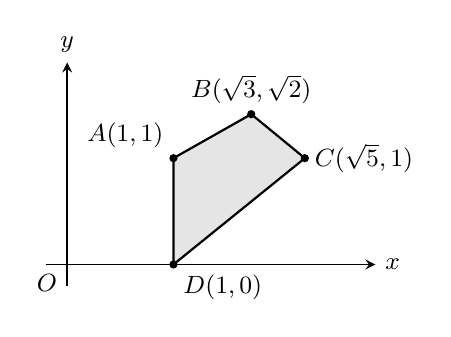
\begin{tikzpicture}[>=stealth, semithick, font=\small, scale=1.35]
  \fill[gray!20] (1,0)--(1,1)--(1.732,1.414)--(2.236,1)--cycle;
  \draw[thick] (1,0)--(1,1)--(1.732,1.414)--(2.236,1)--cycle;
  \draw[->] (-0.2,0)--(2.9,0) node[right] {$x$};
  \draw[->] (0,-0.2)--(0,1.9) node[above] {$y$};
  \fill (1,1) circle (1.1pt) node[above left] {$A(1,1)$};
  \fill (1.732,1.414) circle (1.1pt) node[above] {$B(\sqrt3,\sqrt2)$};
  \fill (2.236,1) circle (1.1pt) node[right] {$C(\sqrt5,1)$};
  \fill (1,0) circle (1.1pt) node[below right] {$D(1,0)$};
  \node[below left] at (0,0) {$O$};
\end{tikzpicture}
